\section{ICA Tool}

The ICA tool (\verb!icatool!) performs blind source separation on multiple audio
input files by applying independent component analysis to the corresponding time
signals. Possible choices for the output of the results are either WAVE audio
files or Weka ARFF format.

The format of the input files may differ\footnote{Generally speaking, all audio
  file formats supported by the SDL\_sound library can be read.}, yet all of them
must have the same sampling rate and equal number of samples. Should the latter
vary, the corresponding signal can be expanded by using the expected value of
its time signal.

Whenever an input file contains more than one channel, only the first one will
be used for computation.

If the number of sources to be separated is smaller than the number of input
files, the corresponding number of signals with the greatest variance and thus
most information will be selected from all available signals. Since principal
component analysis is a preprocessing step for ICA anyway, this yields no
particular further computational effort.\\

Readers should note that this is a stand-alone application that makes no further
use of the framework's storage- and/or classification components.


\paragraph{General}

\begin{itemize}
  \item {\tt --help} -- display information about command line parameters and
    exit.
  \item {\tt --as-wave} -- output the results as WAVE audio files, which is
    also the default.
  \item {\tt --as-arff} -- output the results as Weka ARFF files.
  \item {\tt --prefix=<prefix>} -- the prefix to be used for the output
    files. The filenames will be comprised of \verb!<prefix><nr>.<format>!,
    where \verb!<nr>! equals the number of each separated source and
    \verb!format!  resembles the chosen output file format.
\end{itemize}

\paragraph{Separation}

\begin{itemize}
  \item {\tt --nsources=<x>} -- the number of sources to be separated. Must be
    greater one and less than or equal to the number of input files.
  \item {\tt --force} -- in case of varying lengths of the input signals,
    extends shorter input signals by their expected values instead of aborting.
  \item {\tt --prec=<x>} -- the desired precision for the projection of the
    components. Must be a real value greater than $10^{-20}$. Defaults to
    $10^{-10}$.
  \item {\tt --max-iter=<x>} -- the maximum number of iterations per component
    for FastICA. Applies only if the desired precision has not been achieved
    before reaching this limit.
\end{itemize}


\subsubsection{Usage Examples}

\begin{itemize}
  \item {\tt icatool --prefix=foo mix31.wav mix32.wav mix33.wav}\\
    Performs ICA on the given input files and outputs the results as WAVE audio
    files with the names {\tt foo1.wav}, {\tt foo2.wav} and {\tt foo3.wav}.
  \item {\tt icatool --as-arff --prefix=baz mix4[1-4].wav}\\ 
    Performs ICA on the four given input files {\tt mix41.wav} to {\tt
    mix44.wav} and outputs the results in Weka ARFF format with the names {\tt
    baz1.arff} to {\tt baz4.arff}.
  \item {\tt icatool --prefix=ext --force shorter.mp3 longer[1-2].mp3}\\
    Performs ICA on the three given input files, one of which has less samples
    than the others. The time signal of the ``delinquent'' is expanded by its
    expected value. Output will be as WAVE audio files with the names {\tt
      ext1.wav} to {\tt ext3.wav}.
  \item {\tt icatool --prefix=reduced --nsources=2 mix5[1-5].ogg}\\
    Performs ICA on the five given input files {\tt mix51.ogg} to {\tt
      mix55.ogg} and output the results as WAVE audio files. Before the actual
    application of ICA, however, the two principal signals, i.e. the signals
    with the greatest variance and thus most information, are selected amongst
    all available signals.
\end{itemize}


\subsection{Separation Tool}
\label{section:septool}

The separation tool (\verb!septool!) is the central command-line application of
openBliSSART. It takes one or more audio files and separates
them into components by using non-negative matrix factorization.  Components can
be stored and/or classified using an existing response variable.\\
In the former case, each component is saved to the database as classification
object. Also, the parameters of the separation process are saved.\\
In the case of classification, an audio file is generated for each class.\\

An arbitrary number of files to be processed ($\geq 1$) can be given as
arguments. WAV and MP3 formats are supported.\footnote{Generally speaking, all
  audio file formats supported by the SDL\_sound library can be read.}
Furthermore, the process can be controlled via a variety of parameters,
are listed below.

\paragraph{General}

\begin{itemize}
  \item {\tt -h}, {\tt --help} -- display information about command line
    parameters and exit.
  \item {\tt -A}, {\tt --echo} -- print the base name of the application binary
    and its named command line options in long format, with their parameters if 
    given, before executing.
  \item {\tt -C}, {\tt --config=<filename>} -- use the specified configuration
    file (properties format) instead of the default one. See section 
    \ref{section:ConfigFiles} for details.
  \item {\tt -n<number>}, {\tt --num-threads=<number>} -- the number of
    concurrent threads to use for separation and classification. Should be set
    to the number of CPUs (cores) present in the computer for maximum
    performance.
  \item {\tt -S}, {\tt --scripted} -- run in ``scripted'' mode, i.e. assume that
    the input files contain file names of audio files separated by
    newlines. This option can be useful if lots of files should be processed,
    and to ensure compatibility with systems that limit the number of
    command-line options.
\end{itemize}

\paragraph{Audio Preprocessing}

Transformation options given on the command line override the corresponding 
configuration options (see \ref{section:ConfigFileAudio}).

\begin{itemize}
  \item {\tt -r<function>}, {\tt --reduce-mids} -- subtract right from left
    channel when converting from a stereo to a mono signal.
  \item {\tt -k<k>}, {\tt --preemphasis=<k>} -- preemphasizes the signal with
    a factor of $k$ such that for all $t > 0$, $s_t' = s_t - ks_{t-1}$, where
    $s_t$ and $s_t'$ are the sample values at position $t$ in the original and
    preemphasized signal, respectively.
  \item {\tt -d}, {\tt --remove-dc} -- subtracts the mean (DC component) from
    each frame before transformation.
\end{itemize}

\paragraph{Transformation}

Transformation options given on the command line override the corresponding 
configuration options (see \ref{section:ConfigFileFFT}).

\begin{itemize}
  \item {\tt -w<function>}, {\tt --window-function=<function>} -- the window
    function to use in short-time Fourier transformation. Must be one of
    ``hann'' (Hann function), ``sqhann'' (Square root of the Hann
    function), ``hamming'' (Hamming function) or ``rectangle'' (rectangle
    function). The default is ``sqhann''.
  \item {\tt -o<overlap>}, {\tt --overlap=<overlap>} -- overlap of windows,
    given as a number from the interval [0,1). The default is 0.5.
  \item {\tt -s<size>}, {\tt --windowSize=<size>} -- window size in
    milliseconds. Default is 25.
  \item {\tt -z}, {\tt --zero-padding} -- perform zero-padding before FFT,
    such that the transformation size is a power of 2.
\end{itemize}

\paragraph{Separation}

\begin{itemize}
  \item {\tt -m<method>}, {\tt --method=<method>} -- The method to be used
    for component separation. As of the time of writing, this option exists
    only for extensibility reasons and has no effect.
  \item {\tt -c<number>}, {\tt --components=<number>} -- The number of
    components which should be separated. Default is 20.
  \item {\tt -T<number>}, {\tt --spectra=<number>} -- The number of spectra
    which should be computed per component. If the number of spectra is > 1,
    NMD is performed. Default is 1.
  \item {\tt -f<name>}, {\tt --cost-function=<name>} -- The cost function for
    NMF/NMD. The following strings are valid: ``ed'' (Euclidean distance),
    ``kl'' (Kullback-Leibler divergence) \cite{LeeSeung2001}, ``eds'' (Euclidean distance with a 
    sparsity constraint), ``eds'' (Euclidean distance with a sparsity constraint),
    ``kls'' (KL divergence with a sparsity constraint) \cite{Virtanen2007} and finally ``edsn'' 
    (Euclidean distance with a sparsity constraint, measured using normalized
    basis vectors as in \cite{Eggert2004}). Default is ``kl''. Note that NMD
    (i.\,e.\ > 1 spectrum per component) can only be performed using the ``ed''
    and ``kl'' cost functions.
  \item {\tt -y<number>}, {\tt --sparsity=<number>} -- The sparsity parameter
    for the NMF cost function. Only has an effect if either ``eds'', ``edsn''
    or ``kls'' are selected as cost function.
  \item {\tt -N}, {\tt --normalize-matrices} -- Normalize NMF/NMD matrices such
    that the second factor has unity Frobenius norm.
  \item {\tt -g}, {\tt --generator=<func>} -- Sets the generator function for
    initialization of the matrices (``gaussian'' for absolute Gaussian noise, 
    ``uniform'' for values uniformly distributed on the interval $[0.01,0.02)$,
    or ``unity'' for every value equal to 1). Default is ``gaussian''.
    The ``unity'' generator makes the separation process deterministic and can
    hence be used for debugging purposes.
  \item {\tt -e<number>}, {\tt --precision=<number>} -- The desired precision
    (relative error in terms of Frobenius norm) of the result. If set to zero,
    the maximum number of iteration steps is performed in any case. Default is
    0.
  \item {\tt -i<number>}, {\tt --max-iter=<number>} -- The maximum number of
    iteration steps. Default is 100.
  \item {\tt -I<range>}, {\tt --init=<range>} -- Pre-initializes the
    separation using the spectra of several classification objects,
    specified as a range of classification object IDs. ``range'' is a
    string of the form ``min..max'' where ``min'' and ``max'' are IDs of
    classification objects. This option can be repeated to specify multiple
    ranges. If the number of initialization objects is smaller than the
    number of components, randomized spectra are added. The option can be 
    repeated to give multiple ranges of objects for initialization.
  \item {\tt -P}, {\tt --preserve} -- preserves the initialization, i.e. do
    not update it during iteration. Nevertheless, if the number of
    initialization objects is smaller than the number of components, the
    additional randomized are updated in any case.
\end{itemize}

\paragraph{Component Processing}
\begin{itemize}
  \item {\tt -v}, {\tt --volatile} -- run in ``volatile'' mode,
    i.e. components are thrown away after the tool terminates. This only makes
    sense when either the {\tt classify} or one of the ``export'' options are
    activated. If the {\tt --volatile} option is \emph{not}
    specified, components are stored for later use.
  \item {\tt --export-prefix=<prefix>} -- sets the filename prefix for export of
    components (as WAV files) or matrices.
  \item {\tt -p<prefix}, {\tt --export-components} -- exports the separated
    components as WAV files with the given prefix.
  \item {\tt --export-matrices=<name>} -- Export the separation matrices. 
    {\tt <name>} can be one of ``W'' (spectra, first factor), 
    ``H'' (gains, second factor) or ``WH'' (both factors, not the product!)
    The export format is controlled by the {\tt blissart.separation.export.format}
    configuration option (see Section \ref{section:ConfigFiles}).
  \item {\tt -l<response>}, {\tt --classify=<response>} -- performs feature
    extraction on the separated components, classifies them using training
    data from the given response, and generates audio files for each class
    which are named like {\tt <input\_file\_name>\_<class\_name>.wav}.
  \item {\tt -L<label>}, {\tt --preset-label=<label>} -- during classification,
    assigns the label with the given ID to the components which have been 
    initialized by the {\tt -I} option, instead of the class label predicted 
    by the classifier.
\end{itemize}


\subsubsection{Usage Examples}

\begin{itemize}
  \item {\tt septool file.wav} \\
    Separates {\tt file.wav} into 20 components using the default NMF settings,
    and saves the components.
  \item {\tt septool -c30 -s60 -l7 test.wav}\\
    Separates {\tt test.wav} into 30 components, using a window size of 60 ms,
    saves the components and classifies them using the response with the ID
    7. Assuming this response contains classes ``Class1'' and ``Class2'', files
    named {\tt test\_Class1.wav} and {\tt test\_Class2.wav} are generated.
  \item {\tt septool -v -c30 -s60 -l7 test.wav}\\
    Like the above, except that separated components are not stored.
  \item {\tt septool -n4 file1.wav file2.wav file3.wav file4.wav
      file5.wav}\\
    Separates the files {\tt file1.wav} to {\tt file5.wav} using default
    settings and saves the components, using at most 4 concurrent threads.
  \item {\tt septool -v -T5 -c40 -l7 -I11..30 -P -L3 test.wav}\\
    Separates {\tt test.wav} by means of NMD into 40 components
    ({\tt -c 40}), each consisting of 5 spectra ({\tt -T5}). Thereby the first
    20 are initialized using the classification objects with IDs 11 to 30,
    which must in turn be NMD components ({\tt -I11..30}). Spectra are not
    updated during the iteration ({\tt -P}).  Classification is done using the
    response with ID 7 ({\tt -l7}), where the first 20 components are assigned
    the label with ID 3 regardless of the classifier's decision ({\tt -L3}).
    Nothing is written to the database ({\tt -v}).
  \item {\tt septool -v -T20 -c10 -ptestcomp test.wav}\\
    Separates {\tt test.wav} by means of NMD into 10 components, consisting 
    of 20 spectra each. The components are exported as WAV files with the 
    prefix {\tt testcomp}.
  \item {\tt septool -v -I1..20 -P -c20 --export-matrices=H test.wav}\\
    Separates {\tt test.wav} into 20 components whose spectra are all 
    predefined in the classification objects with IDs 1 to 20.
    The gains matrix (H) is exported to a file.
  \item {\tt septool --cost-function=kls -y0.5 test.wav}\\
    Like the first example, but using sparse NMF, 
    setting the sparsity parameter to 0.5.
\end{itemize}


\subsubsection{Multithreading vs. Multiple Processes}
\label{section:MultithreadingMultiprocessing}

\begin{leftbar}
  It is important to note that while there is an option to run multiple threads
  simultaneously from one single instance of the separation tool (in this case,
  only one \emph{user process} is created by the operating system), starting
  multiple concurrent instances of the separation tool (and hence multiple user
  processes) can lead to errors, as the integrated SQLite database can
  only be written by one user process at a time.
\end{leftbar}


\subsection{Feature Extraction Tool}
\label{section:fextool}

The feature extraction tool (\verb!fextool!) extracts features from stored
components and saves them into the database.

\noindent It can be controlled via the following command line options:
\begin{itemize}
  \item {\tt -h}, {\tt --help} -- only display information about command line
    parameters.
  \item {\tt -A}, {\tt --echo} -- print the base name of the application binary
    and its named command line options in long format, with their parameters if 
    given, before executing.
  \item {\tt -C}, {\tt --config=<filename>} -- use the specified configuration
    file (properties format) instead of the default one. See section 
    \ref{section:ConfigFiles} for details.
  \item {\tt -a}, {\tt --all} -- performs feature extraction for all
    components whose data is available.
  \item {\tt -p<id>}, {\tt --process=<id>} -- performs feature extraction on
    the components that have been generated by the separation process with the
    given ID.
  \item {\tt -n<number>}, {\tt --num-threads=<number>} -- the number of
    concurrent threads to use for separation and classification. Should be set
    to the number of CPUs (cores) present in the computer for maximum
    performance.
\end{itemize}

The feature extraction process itself can be influenced by a great variety of
configuration options, which are all listed in section
\ref{section:ConfigFileFex}.

The same note about multithreading and multiple instances of the tool applies as
for the separation tool (\ref{section:MultithreadingMultiprocessing}).


\subsection{Cross-Validation Tool}

The cross-validation tool ({\tt cvtool}) performs stratified cross-validation of
a data set given by a response.

\noindent The following options can be specified on the command line:
\begin{itemize}
  \item {\tt -h}, {\tt --help} -- displays information about command line
    parameters.
  \item {\tt -A}, {\tt --echo} -- print the base name of the application binary
    and its named command line options in long format, with their parameters if 
    given, before executing.
  \item {\tt -C}, {\tt --config=<filename>} -- use the specified configuration
    file (properties format) instead of the default one. See section 
    \ref{section:ConfigFiles} for details.
  \item {\tt -r<id>}, {\tt --response=<id>} -- gives a response ID. All
    classification objects that are assigned a label in this response are
    validated.
  \item {\tt -f<n>}, {\tt --fold=<n>} -- gives the number of folds. If 0 is
    given, leave-one-out cross-validation is performed. The default value is
    10.
  \item {\tt -t<id>}, {\tt --train=<id>} -- gives a response ID for a
    training set instead of performing $n-$fold cross-validation.
  \item {\tt -s}, {\tt --shuffle} -- shuffles the data set before validation,
    i.e. randomly reorders the classification objects within the data set. Of
    course, this does not make sense for leave-one-out cross-validation.
  \item {\tt --fs=<algorithm>} -- enables automatic feature selection. If {\tt
      algorithm} is {\tt anova}, features are rated by their $t$-test score
    (only available for responses with two classes).  Otherwise, if {\tt
      algorithm} is {\tt correlation}, features are rated by their correlation
    with their class label.
  \item {\tt -m<number>}, {\tt --max-features=<number>} -- gives the maximum
    number of features that automatic feature selection should select.  The
    default value is 10.
  \item {\tt -v}, {\tt --verbose} -- enables verbose output (see below).
  \item {\tt -p}, {\tt --prob} -- estimates probabilities for SVM
    classification. If this option is given, verbose output is automatically
    enabled.
  \item {\tt --dump[=<prefix>]} -- for each fold, write the training and test
    data to an ARFF data file with the given prefix (default prefix: {\tt
      fold}). These files can be used to manually reproduce the
    cross-validation result with the Weka \cite{Weka} software.
\end{itemize}

If a response ID was specified, the tool outputs the number of classification
objects that were validated, the recalls for each class, the mean recall, as
well as the overall accuracy. Finally, a confusion matrix for all classes in the
response is printed.

If verbose output is enabled, additionally a list of misclassified objects,
their ID, their class label, their predicted class label and, if the
corresponding option is given, their prediction probabilities is printed.

Unless automatic feature selection is enabled, the features to be used for
classification are read from the configuration file (see section
\ref{section:ConfigFileFex}).


\subsubsection{Usage Examples}

\begin{itemize}
  \item {\tt cvtool -r7 -f3}\\
    Validates the response with ID 7 using stratified 3-fold cross validation
    and the feature set given by the configuration file.
  \item {\tt cvtool -r7 -t8}\\
    Validates each object in the response with ID 7, using the response with ID
    8 as training set.
  \item {\tt cvtool -r7 --fs=anova -m10 -p}\\
    Validates the response with ID 7 using stratified 10-fold cross validation,
    using the 10 features which score best in a $t$ test, and outputs all
    objects which have been misclassified along with the classification
    probability.
\end{itemize}


\subsection{Export Tool}

The export tool ({\tt export}) exports objects (usually NMF components)
in the storage to a file.
HTK or Gnuplot output format can be selected.

\noindent The following options can be specified on the command line:
\begin{itemize}
  \item {\tt -h}, {\tt --help} -- displays usage information.
  \item {\tt -a}, {\tt --all} -- exports the data from all data descriptors of
    the given type ({\tt -t}) in the database.
  \item {\tt -p<list>}, {\tt --process=<list>} -- exports data descriptors 
    associated with the given process IDs. Single process IDs or ranges 
    ({\tt x..y}) can be given and must be separated with commata.
  \item {\tt -f<format>}, {\tt --format=<format>} -- selects an output format.
    Must be one of ``htk`` or ``gnuplot''. Default is ``htk''.
  \item {\tt -c}, {\tt --concat} -- concatenates data descriptors of the same
  type, so that only one output file per type is generated.
  The type of concatenation (column- or row-wise) depends on the type of
  data descriptor: Spectra are considered column vectors, hence concatenated
  column-wisely; conversely, gains are considered row vectors, hence
  concatenated row-wisely. Magnitude and phase matrices are concatenated
  column-wisely.
  \item {\tt -t<type>}, {\tt --type=<type>} -- selects the type of data
  descriptor to export. Available types are: Spectrum (``spect''), Gains
  (``gains''), Magnitude Matrix (``mmatr''), and Phase Matrix (``phase'').
  \item {\tt --strip-prefix=<path>} -- when selecting the output file name, the
  default is to use the full path name of the corresponding input file is used.
  This option can be used to strip a certain path prefix, to create relative
  file names.
  \item {\tt --target-dir=<path>} -- sets the target directory for output.
  Output files are placed in this directory, and relative path names are
  interpreted with respect to this directory.
  \item {\tt -T}, {\tt --add-type} -- adds a string giving the type of data to
  the file names, e.\,g.\ ``spect''.
\end{itemize}


\subsubsection{Usage Example}

{\tt export -p17 -fgnuplot -tgains -c}\\
Exports the gains vectors created in
process 17 and concatenates them. The output (in this case a gains matrix) 
is written to a file in Gnuplot format.


\subsection{Audio Export Tool}

In contrast to the export tool, the audio export tool ({\tt exportaudio})
exports objects (usually NMF components) in the storage to an audio file.
\noindent The following options can be specified on the command line:
\begin{itemize}
  \item {\tt -h}, {\tt --help} -- displays usage information.
  \item {\tt -o<id1>[..<id2>]}, {\tt --object-id=<id1>[..<id2>]}
    -- selects the objects to export. Single IDs or ranges of IDs can be given.
    This option can be repeated to export multiple objects or ranges.
\end{itemize}


\subsection{Cleanup Tool}

Because openBliSSART stores binary data in a filesystem directory which is
physically independent of the database, there exist some cases where
`orphaned' binary files remain in the storage directory, without a data
descriptor referencing them.

The purpose of the cleanup tool ({\tt cleanup}) is to purge the storage
directory of these files. After execution, it displays the number of files that
have been deleted.

The {\tt -s} or {\tt --simulate} option can be used if no deletions should
be performed, but just the number of ``orphaned'' files should be printed.


\subsection{Browser}
\label{section:browser}

The main purpose of the browser application is to facilitate the creation
of data sets (responses) which can be used for classification of NMF components
in blind source separation. It also supports playback of components,
displays component features and allows export of selected
data sets to Weka \cite{Weka} for a more detailed assessment of suitability.

The user interface has been designed with simplicity in mind, i.e. having
everything at hand where it might be needed or helpful. Thus, the database
entities are displayed in a tree-like view on the main window's left-hand side.
Further information related to any entity can be displayed by simply expanding
the corresponding subtree. For an example, refer to figure
\ref{figure:ExpandedSubtree}.

Also, when selecting a database entity, edit and/or preview facilities will be
provided on the user interface's right-hand side, the so-called \emph{edit
  area}. Furthermore, almost every item provides a context-sensitive menu that
shows up when the user presses the right mouse button on an item.

\begin{figure}
    \centering
    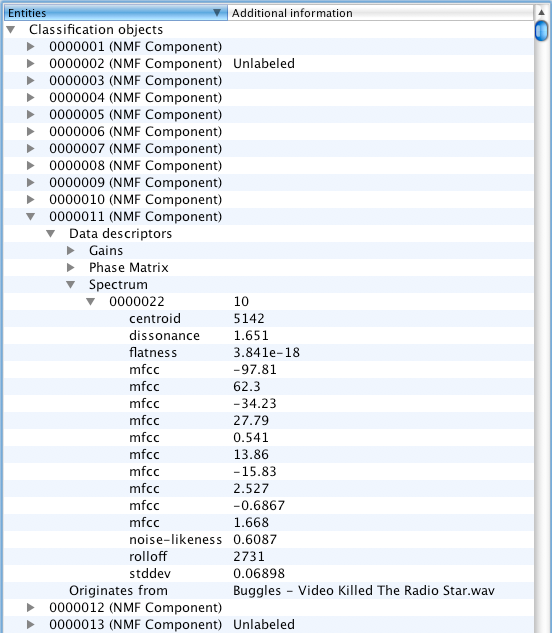
\includegraphics[width=.5\textwidth]{images/ExpandedSubtree.png}
    \caption{%
        \label{figure:ExpandedSubtree}%
        Example subtree expansion
    }
\end{figure}


\subsubsection{Typical Workflow}

For example, a typical workflow could be
\begin{itemize}
  \item   the creation of a number of separation processes, followed by
  \item   the extraction of the related features, followed by
  \item   the creation of various labels with arbitrary precision, followed by
  \item   the assignment of one or more labels to selected classification
    objects, followed by
  \item   the creation of one or more responses, followed by
  \item   the assignment of classification objects to one or more responses
    and finally
  \item   the evaluation of a response.
\end{itemize}


\subsubsection{Import of Audio Files}

Figure \ref{figure:ProcessCreation} shows an example of the ``Import audio''
dialog. This dialog can be displayed either by pressing the respective button or
by selecting the corresponding entry from the application's main menu, or
alternatively the context menu of the tree view.

\begin{figure}
    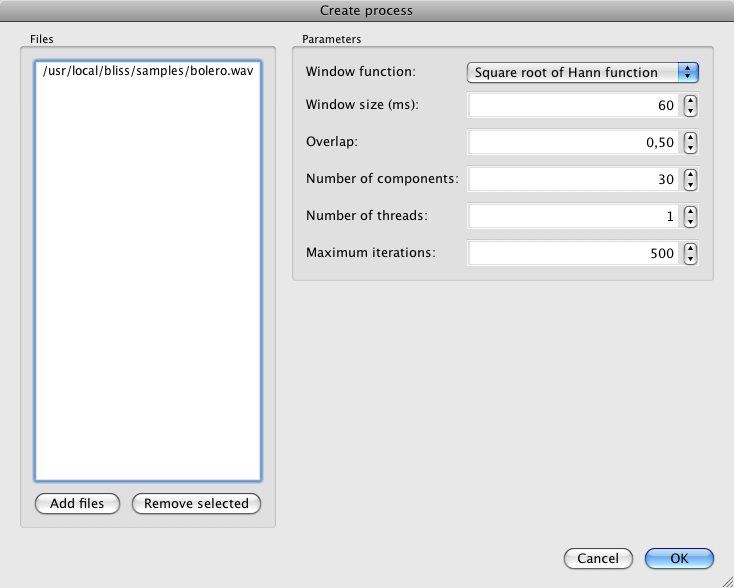
\includegraphics[width=\textwidth]{images/ProcessCreation.png}
    \caption{%
        \label{figure:ProcessCreation}%
        Example audio import dialog
    }
\end{figure}

While an arbitrary number of input files can be specified on the left-hand side,
the right-hand side allows the selection of the intended parameters for the
separation process. Currently only a subset of the parameters of the separation
tool is offered by the browser.

Note that increasing the number of threads is only useful when working with
multiple files because they will be distributed individually among the available
worker-threads. Also, the number of threads should not exceed the number of
available processors as there are only few disk operations but rather heavy
computational costs involved in the separation process.


\subsubsection{Feature Extraction}

While it is possible to extract the features of individual classification object
(see figure \ref{figure:FeatureExtraction}) via their context menu, the features
of all classification objects can be extracted in one step as well by selecting
the appropriate item from the application' menu.

Again, the number of threads can be specified when extracting all features at
once and significantly reduces the processing time on multiprocessor machines.

\begin{leftbar}
    If you change the configuration options for feature extraction (see
    \ref{section:ConfigFileFex}), you have to restart the browser for changes to
    take effect.
\end{leftbar}

\begin{figure}
    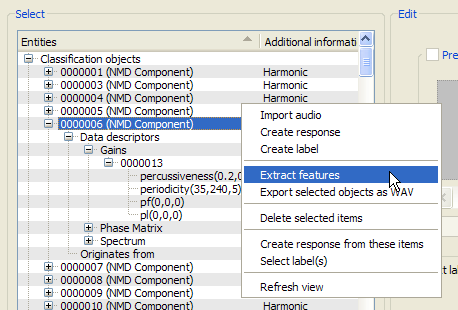
\includegraphics[width=\textwidth]{images/FeatureExtraction.png}
    \caption{%
        \label{figure:FeatureExtraction}%
        Feature extraction
    }
\end{figure}


\subsubsection{Label Creation}

Labels can be created either by pressing the corresponding ``Create label''
button located at the user interface's lower left or by selecting the
appropriate item from the application's or context menu. Creating a label
automatically inserts the new label into the tree view, selects it and allows
editing of the label's properties inside the edit area.


\subsubsection{Assignment of Labels to Classification Objects}

After a suitable set of labels has been created, these labels have to be
assigned to classification objects wherever appropriate. Selecting a
classification object shows a list of all available labels inside the edit
area. One or more labels can be assigend by checking the corresponding checkbox
and then saving this selection. Figure \ref{figure:LabelAssignment} shows the
selection of multiple labels for a particular classification object.  In order
to determine which of the available labels satisfy the needs of a particular
classification object, one can use the application's preview feature so as to
visually explore the samples or else playing them back. Depending on the
applications preferences, the ``Preview'' checkbox is checked automatically. If
not, either manually check that box to be able to explore the samples or select
the corresponding option in the preferences dialog.

\begin{figure}
    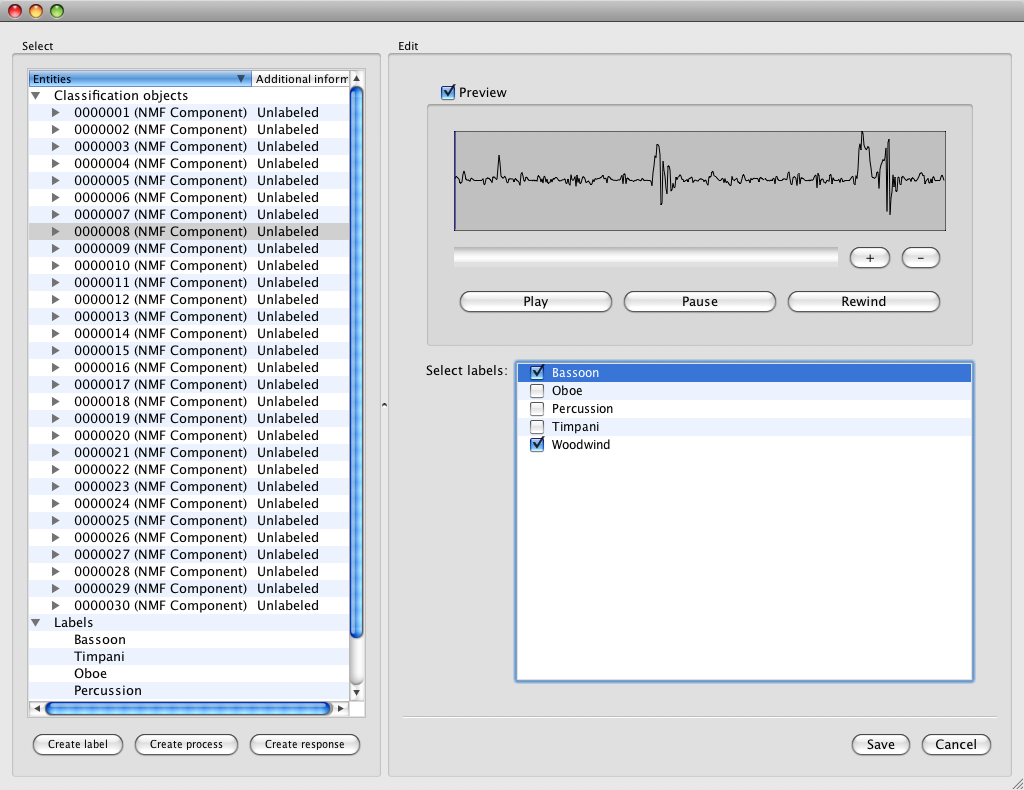
\includegraphics[width=\textwidth]{images/LabelAssignment.png}
    \caption{%
        \label{figure:LabelAssignment}%
        Assignment of labels to classification objects
    }
\end{figure}

It is also possible to select one or more labels for multiple classification
objects at once by means of the ``Select label'' item in their context menu. In
this case, a dialog is shown which allows the selection of one or more
labels. The selected labels are assigned to each selected classification
object. Existing labels are not removed.


\subsubsection{Response Creation}

To create an empty response, either press the ``Create response'' button located
at the user interface's lower left or select the corresponding item from the
main menu or the context menu of the tree view.  The newly created response is
automatically inserted into the entities tree while the response's properties
(name, description and assigned classification objects) can be modified inside
the edit area.

To create a response that contains a set of classification objects, simply
select the desired classification objects in the tree view and click ``Create
response from these items'' in the context menu.


\subsubsection{Adding Classification Objects to Responses}

Currently the only way to assign classification objects to an existing response
is via the ``Add CLO's by label'' button located inside a response's edit area.
Pressing this button pops up a dialog that allows the selection of the desired
label. Thereupon all classification objects related to this label will be
assigned to the current response.

Since multiple labels can be assigned to a classification object, one might wish
to change the label in-use. In order to do that, simply select the corresponding
classification object from the list inside the response's edit area and press
``Select label''. Note that this button will be enabled as soon as \emph{more
  than one} label is linked to the selected classification object.

Classification objects can be removed from the assignment list by selecting them
followed by pressing the ``Remove selected'' button.

As with all of the browser's edit options, the newly made assignments are not
automatically stored. Instead, they have to be saved explicitly.

Figure \ref{figure:COAssignment} shows the described features.

\begin{figure}
    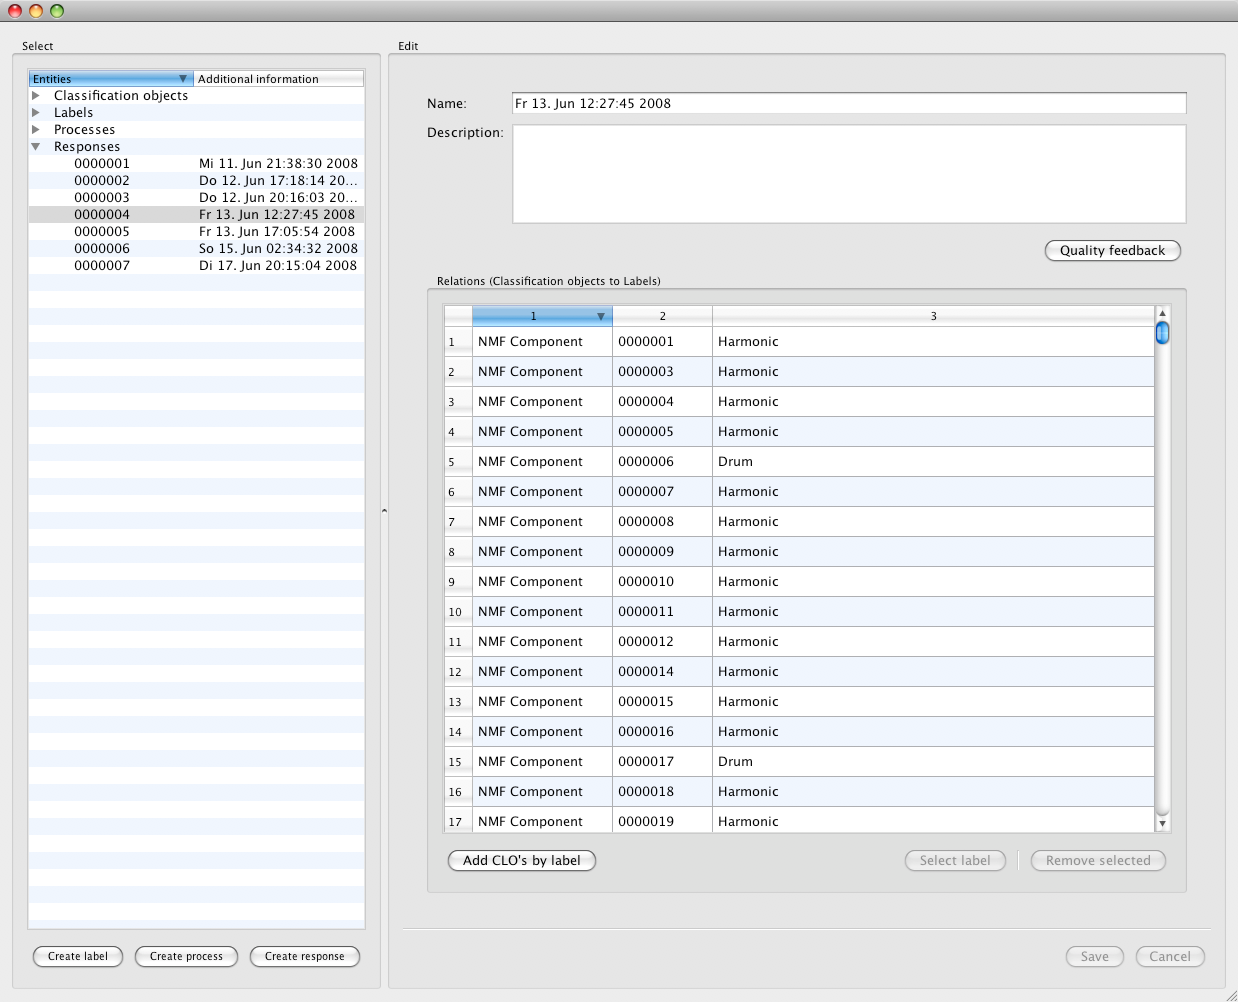
\includegraphics[width=\textwidth]{images/COAssignment.png}
    \caption{%
        \label{figure:COAssignment}%
        Assignment of classification objects to a response
    }
\end{figure}


\subsubsection{Response Evaluation}

Like mentioned before, the application provides a way of evaluating a response's
quality and/or, for an even more detailed exploration, exporting all features
related to the response's assigned classification objects to Weka.  This can be
achieved by pressing the ``Quality feedback'' button, which automatically shows
a dialog that calculates and displays all expected values and variances of the
associated features. An example is shown in figure \ref{figure:QualityFeedback}.

Pressing the dialog's ``Export to Weka'' button exports the corresponding data
to a selected file in Weka's ARFF format. For a detailed description of this
file format, please refer to \cite{Weka}.

\begin{figure}
    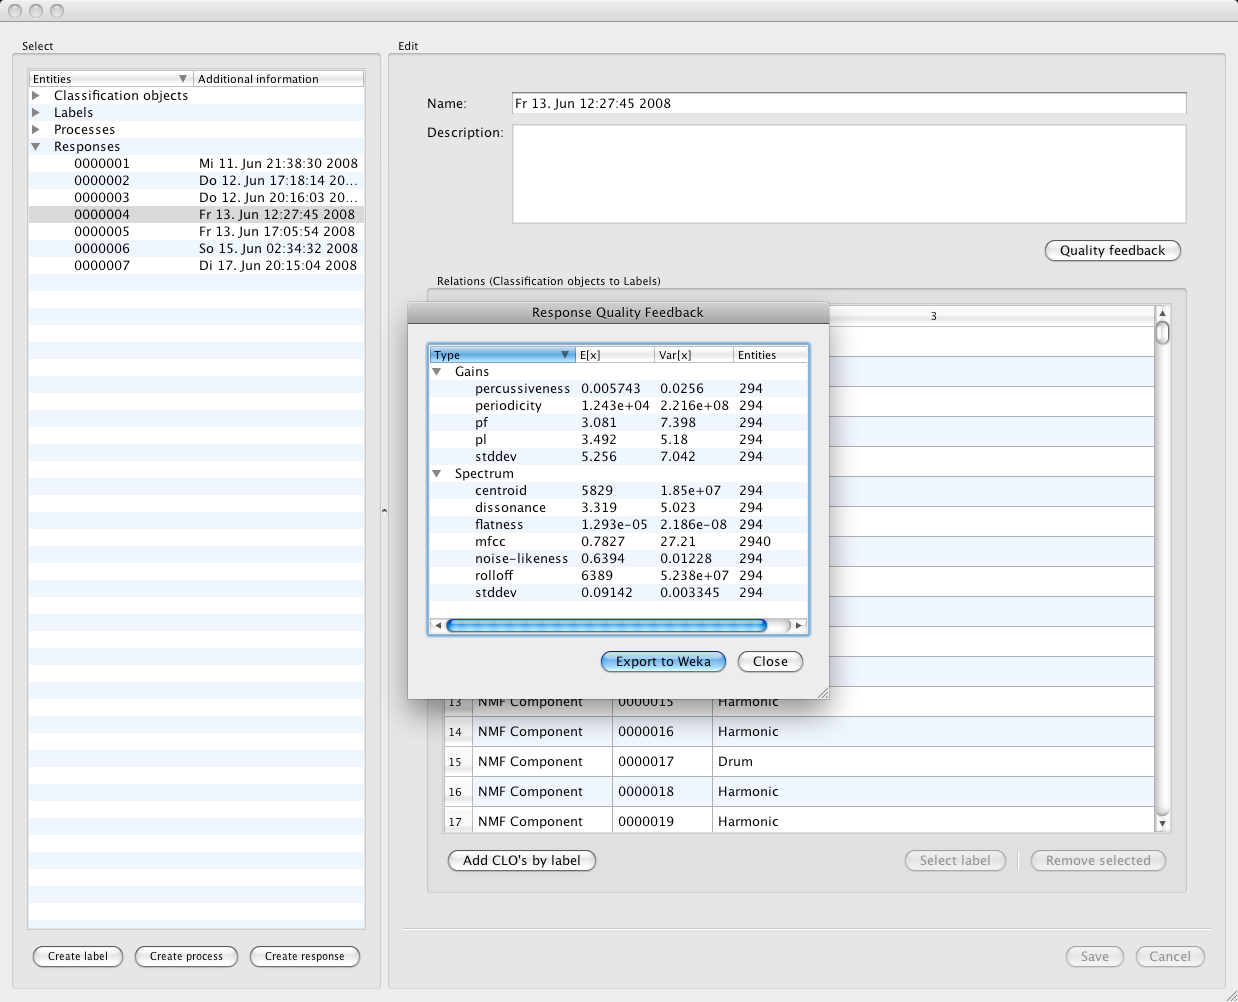
\includegraphics[width=\textwidth]{images/QualityFeedback.png}
    \caption{%
        \label{figure:QualityFeedback}
        Response evaluation
    }
\end{figure}


\subsubsection{Exporting selected Classification Objects}

If a selection of classification objects should be exported as audio files, one
can simply select the desired objects and choose ``Export selected components''
via the corresponding objects' context menu item. When selecting this item, a
directory selection dialog shows up and allows selecting the destination
directory for the exported files.


\subsection{Configuration Files}

\label{section:ConfigFiles}

Audio processing, feature extraction, classification and browser behavior can be
fine-tuned by means of configuration files in the Java properties file
format. Basically, files in this format may contain option lines of the form

\centerline{\tt <option-name>: <option-value>}

as well as comment lines starting with {\tt \#}, which are ignored. Boolean
values can be notated as {\tt 0}, {\tt false} or {\tt 1}, {\tt true},
respectively.\\

The configuration files reside in the {\tt etc} directory of the installation
tree.


\subsubsection{Global Options}
\label{section:ConfigFileGlobal}

\begin{itemize}
  \item   {\tt blissart.global.mfcc.count} (positive integer): The number of
    Mel frequency cepstral coefficients (MFCCs) to compute. Default is 13.
  \item   {\tt blissart.global.mfcc.mfcc0} (boolean): Whether the first MFCC
    should be computed. Default is {\tt true}. If this option is set to {\tt
    false} and {\tt blissart.global.mfcc.count} is set to $N$, MFCCs 1 through 
    $N-1$ are computed.
  \item   {\tt blissart.global.mfcc.lifter} (double): The parameter for MFCC
    liftering. Liftering with parameter $L$ means that the $i$th
    coefficient is multiplied with $1 + L / \sin(2\pi i / L)$, i.e. if
    $L=0$ this procedure has no effect. More information can be found in
    the HTK book \cite{HTKBook}.
  \item   {\tt blissart.global.mel\_bands} (positive integer): The number of
    Mel frequency bands to use for Mel filtering (e.g. in MFCC computation).
  \item   {\tt blissart.global.deltaregression.theta} (positive integer): The
    parameter $\theta$ for the regression procedure which is used to
    compute delta- and delta-delta MFCCs. More information can be found in
    the HTK book \cite{HTKBook}.
\end{itemize}


\subsubsection{Audio Preprocessing}
\label{section:ConfigFileAudio}

Audio preprocessing options can be specified in the configuration file {\tt
  blissart.properties}. These are valid for the browser as well as the
separation tool, but can be overridden by passing the corresponding command line
parameters to the separation tool.

\begin{itemize}
  \item {\tt blissart.audio.remove\_dc} (boolean): See the {\tt --remove-dc}
    option of the separation tool.
  \item {\tt blissart.audio.preemphasis}: See the {\tt --preemphasis} option of
    the separation tool.
  \item {\tt blissart.audio.reduce\_mids}: See the {\tt --reduce-mids} option of
    the separation tool.
\end{itemize}


\subsubsection{Transformation}
\label{section:ConfigFileFFT}

Options for the short-time Fourier transformation can be specified in the
configuration file {\tt blissart.properties}. Some of these can be overridden in the
``Import audio'' dialog of the browser, as well as by passing the corresponding
command line parameters to the separation tool. In addition, the short-time
Fourier spectrograms can be transformed in various ways, as will be explained
below.

\begin{itemize}
  \item {\tt blissart.fft.windowfunction} (string): See the {\tt
      --window-function} option of the separation tool.
  \item {\tt blissart.fft.windowsize} (positive integer): See the {\tt
      --window-size} option of the separation tool.
  \item {\tt blissart.fft.overlap} (double): See the {\tt --overlap} option of
    the separation tool.
  \item {\tt blissart.fft.zeropadding} (boolean): See the {\tt --zero-padding}
    option of the separation tool.
  \item {\tt blissart.fft.transformations.powerSpectrum}: 
        If set to {\tt true}, converts the spectrum to the power spectrum (default: square).
  \item {\tt blissart.fft.transformations.powerSpectrum.gamma}: 
        The exponent for the power spectrum (default 2.0).
  \item {\tt blissart.fft.transformations.melFilter}: 
        If set to {\tt true}, applies a Mel filterbank to the spectrogram.
        The number of Mel bands is controlled by the
        {\tt blissart.global.mel\_bands} global option.
  \item {\tt blissart.fft.transformations.slidingWindow}: 
        If set to {\tt true}, applies a `sliding window' to the spectrogram, i.\,e.\ multiple
        columns (frames) are concatenated into a single column.
  \item {\tt blissart.fft.transformations.slidingWindow.frameSize}: 
        The `frame size' for the sliding window transformation, i.\,e.\ the
        number of columns to concatenate for each output column. Default is 10.
  \item {\tt blissart.fft.transformations.slidingWindow.frameRate}: 
        The `frame rate' for the sliding window transformation, i.\,e.\ the
        number of columns to skip between subsequent concatenations.
\end{itemize}
 
  
\subsubsection{Separation}

Options for the separation process can be specified in the
configuration file {\tt blissart.properties}.

\begin{itemize}
  \item {\tt blissart.separation.notificationSteps}:
        The number of iteration steps after which a notification is generated,
        i.\,e.\ the progress bar is updated in the septool and Browser
        applications. Default ist 25. Setting this number to a low value may
        result in performance loss for small input files, whereas raising it
        to a high value prevents any progress begin seen over long periods of
        time.
  \item {\tt blissart.separation.export.format}:
        One of ``bin'', ``htk'' or ``gnu'' for BliSSART binary matrix format,
        HTK format or Gnuplot format, respectively. This option has an effect
        on the separation tool with the {\tt --export-matrices} option enabled.
  \item {\tt blissart.separation.storage.phasematrix}:
        {\tt true} (default) if the separation tool should store the phase
        matrix of the original signal, {\tt false} otherwise.
  \item {\tt blissart.separation.storage.magnitudematrix}:
        {\tt true} if the separation tool should store the magnitude
        matrix of the original signal, {\tt false} otherwise (default).
        Usually this option should be disabled.
\end{itemize}


\subsubsection{Feature Extraction}
\label{section:ConfigFileFex}

Feature extraction options can be found in the configuration file {\tt
  blissart.properties}. Unless stated otherwise, these options are boolean
values which include/exclude certain features in the feature set. By default,
the following features are included, depending on the type of data descriptor:
\begin{itemize}
    \item   Magnitude matrices:
        \begin{itemize}
            \item   (Sampled) MFCCs
            \item   Delta and delta-delta coefficients
            \item   Mean and standard deviation of those coefficients
        \end{itemize}
    \item   Spectra:
        \begin{itemize}
            \item   MFCCs
            \item   Standard deviation
            \item   Spectral centroid
            \item   Spectral rolloff
            \item   Noise-likeness
        \end{itemize}
    \item   Gains vectors:
        \begin{itemize}
            \item   Periodicity
            \item   Peak length
            \item   Peak fluctuation
            \item   Percussiveness
        \end{itemize}
\end{itemize}

The following options control feature extraction from magnitude matrices:
\begin{itemize}
  \item {\tt blissart.features.magnitudematrix.mfcc}: Whether to compute
    MFCCs. MFCCs are sampled at a given number of equidistant frames which can
    be modified by the {\tt blissart.features.magnitudematrix.mfcc.frame\_count}
    option (default 5).
  \item {\tt blissart.features.magnitudematrix.mfccD}: Whether to compute delta
    coefficients (using the regression procedure described in the HTK book
    \cite{HTKBook}).
  \item {\tt blissart.features.magnitudematrix.mfccA}: Whether to compute
    delta-delta ({\bf A}cceleration) coefficients (using the regression
    procedure described in the HTK book \cite{HTKBook}).
  \item {\tt blissart.features.magnitudematrix.mean\_mfcc}: Whether to compute
    the mean of each MFCC over the whole signal.
  \item {\tt blissart.features.magnitudematrix.mean\_mfccD}: Whether to compute
    the mean of each delta coefficient over the whole signal.
  \item {\tt blissart.features.magnitudematrix.mean\_mfcc}: Whether to compute
    the mean of each delta-delta coefficient over the whole signal.
  \item {\tt blissart.features.magnitudematrix.stddev\_mfcc}: Whether to compute
    the standard deviation of each MFCC over the whole signal.
  \item {\tt blissart.features.magnitudematrix.stddev\_mfccD}: Whether to
    compute the standard deviation of each delta coefficient over the whole
    signal.
  \item {\tt blissart.features.magnitudematrix.stddev\_mfccA}: Whether to
    compute the standard deviation of each delta-delta coefficient over the
    whole signal.
\end{itemize}


The following options control feature extraction from spectra:
\begin{itemize}
  \item {\tt blissart.features.spectrum.mfcc}: Whether to compute MFCCs.
  \item {\tt blissart.features.spectrum.stddev}: Whether to compute standard
    deviation.
  \item {\tt blissart.features.spectrum.centroid}: Whether to compute the
    spectral centroid.
  \item {\tt blissart.features.spectrum.rolloff}: Whether to compute spectral
    rolloff.
  \item {\tt blissart.features.spectrum.noiselikeness}: Whether to compute
    noise-likeness (\cite{Uhle2003}).
  \item {\tt blissart.features.spectrum.noiselikeness.sigma}: The $sigma$
    (standard deviation) parameter for the calculation of noise-likeness
    (\cite{Uhle2003}).
  \item {\tt blissart.features.spectrum.dissonance}: Whether to compute spectral
    dissonance (\cite{Uhle2003}).  Be aware that this operation can be
    time-consuming, as its time complexity is quadratic in the length of the
    spectra.
  \item {\tt blissart.features.spectrum.flatness}: Whether to compute spectral
    flatness \cite{Uhle2003}.
\end{itemize}

The following options control feature extraction from gains vectors:
\begin{itemize}
  \item {\tt blissart.features.gains.stddev}: Whether to compute standard
    deviation.
  \item {\tt blissart.features.gains.pl}: Whether to compute peak length
    \cite{Virtanen2005}.
  \item {\tt blissart.features.gains.pf}: Whether to compute peak fluctuation
    \cite{Virtanen2005}.
  \item {\tt blissart.features.gains.percussiveness}: Whether to compute
    percussiveness \cite{Uhle2003}.
  \item {\tt blissart.features.gains.percussivness.length} (double): The length
    (in seconds) of the percussive impulse to use for computation of
    percussiveness.
  \item {\tt blissart.features.gains.periodicity}: Whether to compute
    periodicity of gains \cite{Virtanen2005}.
  \item {\tt blissart.features.gains.periodicity.bpm\_min} (positive integer):
    The minimum bpm (beats per minute) value to consider for periodicity.
  \item {\tt blissart.features.gains.periodicity.bpm\_max} (positive integer):
    The maximum bpm (beats per minute) value to consider for periodicity.
  \item {\tt blissart.features.gains.periodicity.bpm\_step} (positive integer):
    The distance between the bpm values to consider for periodicity.
\end{itemize}


\subsubsection{Classification}
\label{section:ConfigFileClassification}

Classification options control SVM parameters and scaling. They can be specified
in the configuration file {\tt blissart.properties}.

The type of kernel function that is used to build the SVM is given by the {\tt
  blissart.classification.svm.kernel} option. Possible values include {\tt
  linear} for linear functions, {\tt poly} for polynomials of higher degree,
{\tt rbf} for radial basis functions and {\tt sigmoid} for sigmoid functions.
Default is {\tt linear}. The polynomial degree can be given by the {\tt
  blissart.classification.svm.degree} option, which defaults to 3.
       
The precision of the training procedure is controlled by the {\tt
  blissart.classification.svm.epsilon} option (default: $1e-3$).
   
``Bias'' components (i.e. one component that is always 1) can be added by
settings the {\tt blissart.classification.addBias} to {\tt true}.

Scaling is controlled by the {\tt blissart.classification.scaling} family of
options:

\begin{itemize}
  \item {\tt blissart.classification.scaling.method}
    \begin{itemize}
      \item {\tt minmax} for linear scaling such that all values of one feature
        are in a given interval (by default $[-1,1]$),
      \item {\tt musigma} for linear scaling such that all values of one feature
        have the given mean $\mu$ and standard deviation $\sigma$ (by default
        $\mu = 0, \sigma = 1$),
      \item {\tt none} for no scaling.
    \end{itemize}
  \item {\tt blissart.classification.scaling.lower} -- lower bound of the
    scaling interval if {\tt blissart.classification.scaling.method} is set to
    {\tt minmax}.
  \item {\tt blissart.classification.scaling.upper} -- upper bound of the
    scaling interval if {\tt blissart.classification.scaling.method} is set to
    {\tt minmax}.
  \item {\tt blissart.classification.scaling.mu} -- desired mean of the feature
    values if {\tt blissart.classification.scaling.method} is set to {\tt
      musigma}.
  \item {\tt blissart.classification.scaling.sigma} -- desired standard
    deviation of the feature values if {\tt
      blissart.classification.scaling.method} is set to {\tt musigma}.
\end{itemize}
